%%%%%%%%%%%%%%%%%%%%%%%%%%%%%%%%%%%%%%%%%
% Short Sectioned Assignment
% LaTeX Template
%%%%%%%%%%%%%%%%%%%%%%%%%%%%%%%%%%%%%%%%%

%----------------------------------------------------------------------------------------
%	PACKAGES AND OTHER DOCUMENT CONFIGURATIONS
%----------------------------------------------------------------------------------------

\documentclass[paper=a4, fontsize=11pt]{article} % A4 paper and 11pt font size

\usepackage[T1]{fontenc} % Use 8-bit encoding that has 256 glyphs
\usepackage{fourier} % Use the Adobe Utopia font for the document - comment this line to return to the LaTeX default
\usepackage[english]{babel} % English language/hyphenation
\usepackage{amsmath,amsfonts,amsthm} % Math packages

\usepackage{sectsty} % Allows customizing section commands
\allsectionsfont{\raggedright \normalfont\scshape} % Make all sections centered, the default font and small caps

\usepackage{fancyhdr} % Custom headers and footers
\pagestyle{fancyplain} % Makes all pages in the document conform to the custom headers and footers
\fancyhead{} % No page header - if you want one, create it in the same way as the footers below
\fancyfoot[L]{} % Empty left footer
\fancyfoot[C]{} % Empty center footer
\fancyfoot[R]{\thepage} % Page numbering for right footer
\renewcommand{\headrulewidth}{0pt} % Remove header underlines
\renewcommand{\footrulewidth}{0pt} % Remove footer underlines
\setlength{\headheight}{13.6pt} % Customize the height of the header

\usepackage{parskip}
\setlength{\parindent}{15pt}
 \usepackage{graphicx}
\usepackage{caption}
\usepackage{subcaption}
%\numberwithin{equation}{section} % Number equations within sections (i.e. 1.1, 1.2, 2.1, 2.2 instead of 1, 2, 3, 4)
%\numberwithin{figure}{section} % Number figures within sections (i.e. 1.1, 1.2, 2.1, 2.2 instead of 1, 2, 3, 4)
%\numberwithin{table}{section} % Number tables within sections (i.e. 1.1, 1.2, 2.1, 2.2 instead of 1, 2, 3, 4)

\setlength\parindent{0pt} % Removes all indentation from paragraphs - comment this line for an assignment with lots of text

%----------------------------------------------------------------------------------------
%	TITLE SECTION
%----------------------------------------------------------------------------------------

\newcommand{\horrule}[1]{\rule{\linewidth}{#1}} % Create horizontal rule command with 1 argument of height

\title{	
\normalfont \normalsize 
\textsc{Nuclear Engineering, UC Berkeley} \\ [25pt] % Your university, school and/or department name(s)
\horrule{0.5pt} \\[0.4cm] % Thin top horizontal rule
\huge ME 280A Finite Element Analysis \\HOMEWORK 1: THE BASICS  \\  % The assignment title
\horrule{2pt} \\[0.5cm] % Thick bottom horizontal rule
}

\author{Xin Wang} % Your name

\date{\normalsize\today} % Today's date or a custom date

\begin{document}

\maketitle % Print the title

\newpage
\section{Introduction}
The objective of this project is to solve a 1-D differential equation using finite element method. 

\begin{eqnarray}
\frac{d}{dx}(A_1(x) \frac{du}{dx}) &=& f(x)\nonumber\\
f(x)&=&k^2 sin(\frac{\pi kx}{L}) + 2x \nonumber\\
A_1(x)& = &0.2 \nonumber\\
k &= &given constant \nonumber\\
L&=&1 \nonumber\\
u(0)& =& \Delta_1 = given constant =0 \nonumber\\
u(L) &= &\Delta_2 =given constant =1 \nonumber\\
\end{eqnarray}

\section{Analytical solution}
The analytical solution of this equation is easily found after two integrations:

\begin{eqnarray}
A_1 \frac{du}{dx}&=&\int( k^2 sin(\frac{\pi kx}{L}) + 2x ) dx + c_1\nonumber\\
&=& \frac{-Lk cos(\frac{\pi kx}{L})}{\pi} + x^2 +c_1 \nonumber\\
\frac{du}{dx}&=&\frac{1}{A_1}(\frac{-Lk cos(\frac{\pi kx}{L})}{\pi} + x^2 +c_1) \nonumber\\
u(x)&=&\frac{1}{A_1}\int(\frac{-Lk cos(\frac{\pi kx}{L})}{\pi} + x^2 +c_1)dx\nonumber\\
&=&-\frac{1}{A_1}\frac{L^2}{\pi^2} sin(\frac{\pi kx}{L}) + \frac{1}{A_1}\frac{x^3}{3} + c_2x+ c_3
\end{eqnarray}
where $c_1$, $c_2$ and $c_3$ are constants to be determined using boundary conditions. 

For L=1, $A_1$=0.2, the general solution for this equation becomes:
\begin{eqnarray}
u(x)=\frac{-5}{\pi ^2}sin(\pi kx) + \frac{5x^3}{3} + c_2x+ c_3
\end{eqnarray}

The boundary conditions at 0 and L requires:

\begin{eqnarray}
u(0) = c_3 = 0\nonumber\\
u(L) = u(1) =\frac{-5}{\pi ^2}sin(\pi k) + \frac{5}{3} + c_2=1\nonumber\\
c_2= -\frac{2}{3}
\end{eqnarray}

So the solution for the differential equation is:
\begin{eqnarray}
u(x)&=&\frac{-5}{\pi ^2}sin(\pi kx) + \frac{5x^3}{3}  -\frac{2}{3}x \nonumber\\
\frac{du}{dx}&=& \frac{-5k}{\pi} cos(\pi kx) + 5x^2 - \frac{2}{3}
\end{eqnarray}

%%%%%%%%%%%%%%%%%%%%%%%%%%%%%%%%%%%%%%%%%%%%%%%%%%%%%%%%%%%%%%%%%%%%%%%%%%%%%%%%%%%%%%%%%%%
\section{Error}
The error is defined as 

\begin{eqnarray}
e^N = \frac{\| u -u^N \| _{A_1(\Omega)}} {\| u \| _{A_1 (\Omega)}} \nonumber\\
\| u \| _{A_1 (\Omega)} = \sqrt{\int_{\Omega} \frac{du}{dx} A_1 \frac{du}{dx} dx} = \sqrt{\int_{\Omega} A_1(\frac{du}{dx})^2 dx}\nonumber\\
\| u -u^N \| _{A_1(\Omega)} = \sqrt{\int_{\Omega} A_1 (\frac{d(u-u^N)}{dx})^2 dx}
\end{eqnarray}

To compute the error numerically, we calculate the two following quantities element by element, and then assemble them to obtain the overall error:

\begin{eqnarray}
\| u \| _{A_1 (\Omega)}^2 &=&\int_{\Omega} A_1(\frac{du}{dx})^2 dx\nonumber\\
\| u -u^N \| _{A_1(\Omega)} ^2 &=& \int_{\Omega} A_1 (\frac{d(u-u^N)}{dx})^2 dx\nonumber\\
&=& A_1 \int_{\Omega} (\frac{du}{dx} - \frac{du_N}{dx})^2 dx\nonumber\\
&=& A_1 \sum_{e=1}^{N_e} \int_{x_e}^{x_{e+1}} (\frac{du}{dx} - \frac{du_N}{dx})^2 dx \nonumber\\
&=& A_1 \sum_{e=1}^{N_e} \int_{x_e}^{x_{e+1}} (\frac{du}{dx} - \frac{a_{i+1}-a_i}{h_i})^2 dx
\end{eqnarray}

To find the optimal number of elements needed to solve the equation with the acceptable tolerance, the binary search approach is adopted. Starting from as few as two elements, connected at the middle point of the domain, the equation is solved using Finite Element Method and the error computed. If the error doesn't meet the tolerance criteria, then the number of elements is increased by a power of 2. When the error is satisfactory after n iteration, the optimal number of element  should be in the range between $2^{n-1}$ and $2^n$. Based on the result of n, test the error at $(2^{n-1} + 2^n)/2$, if the error is larger than the tolerance, then try the middle point of the right half, and vice versa. 

%%%%%%%%%%%%%%%%%%%%%%%%%%%%%%%%%%%%%%%%%%%%%%%%%%%%%%%%%%%%%%%%%%%%%%%%%%%%%%%%%%%%%%%%%%%%%%%%%%%%%%%%%%%%%%%%%%%
%section Finite Element Method
%%%%%%%%%%%%%%%%%%%%%%%%%%%%%%%%%%%%%%%%%%%%%%%%%%%%%%%%%%%%%%%%%%%%%%%%%%%%%%%%%%%%%%%%%%%%%%%%%%%%%%%%%%%%%%%%%%%

\section{Finite Element Method}

The first step of FEM is to derive the weak form of the differential equation: 

\begin{eqnarray}
\int_{\Omega} \frac{dv}{dx} A_1 \frac{du}{dx} dx = \int_{\Omega} fv dx + A_1 \frac{du}{dx} v \mid _{\partial \Omega}, \forall v
\end{eqnarray}


We approximate the real solution u by

\begin{eqnarray}
u(x) = \sum_{j=1}^{N+1} a_j \phi_j(x)
\end{eqnarray}

and we choose the test function v with the same approximation functions

\begin{eqnarray}
v(x) = \sum_{i=1}^{N+1} b_i \phi_i(x)
\end{eqnarray}

where N is the number of elements and N+1 the number of nodes. 


Then the equation becomes

\begin{eqnarray}
\int_{\Omega} \frac{d}{dx} (\sum_{j=1}^{N+1} a_j \phi_j(x)) A_1 \frac{d}{dx} (\sum_{i=1}^{N+1} b_i \phi_i(x))dx = \int_{\Omega} f (\sum_{i=1}^{N+1} b_i \phi_i(x)) dx + (\sum_{i=1}^{N+1} b_i \phi_i(x) t) \mid _{\Gamma t}, \forall b_i
\end{eqnarray}


As the equation should be valid for any $b_i$, we can regroup the terms into:

\begin{eqnarray}
\sum_{i=1}^{N+1} b_i \int_{\Omega} (\sum_{j=1}^{N+1} a_j \frac{d}{dx} \phi_j(x) A_1 \frac{d}{dx} \phi_i(x)) dx = \sum_{i=1}^{N+1} b_i \int_{\Omega} f \phi_i(x) dx + \sum_{i=1}^{N+1} b_i (\phi_i(x) t) \mid _{\Gamma t}
\end{eqnarray}

We obtain the matrix system to solve:
 
\begin{eqnarray}
K_{ij} &=& \int_{\Omega} \frac{d}{dx} \phi_j(x) A_1 \frac{d}{dx} \phi_i(x) dx \nonumber\\
R_i &=& \int_{\Omega} f \phi_i(x) dx + \phi_i(x) t \mid _{\Gamma t}\nonumber\\
K a &=& R
\end{eqnarray}

A set of basis functions are defined by 

\begin{eqnarray}
\phi_i (x) = \frac{x_i - x_{i-1}}{h_i}, & for &x_{i-1} \leq x \leq x_i \nonumber\\
\phi_i (x) = 1-\frac{x - x_i}{h_{i+1}}, & for &x_{i} \leq x \leq x_{i+1}\nonumber\\
\phi_i (x) = 0 & otherwise
\end{eqnarray}

The derivative of the function is
\begin{eqnarray}
\frac{\phi_i} {dx}  =   \frac{1}{h_i}, & for &x_{i-1} \leq x \leq x_i \nonumber\\
\frac{\phi_i} {dx}  =   \frac{-1}{h_{i+1}}, & for &x_{i} \leq x \leq x_{i+1}\nonumber\\
\frac{\phi_i} {dx}  =     0 & otherwise
\end{eqnarray}

To compute the elements in K and R numerically, we partition the domain into N elements and map the mesh elements to a master element with two shape functions:
\begin{eqnarray}
\hat{\phi_1}     =   \frac{1}{2}(1-\zeta) \nonumber\\
\hat{\phi_2}     =   \frac{1}{2}(1+\zeta)
\end{eqnarray}

The stiffness matrix and the load matrix for element number e are
\begin{eqnarray}
K_{ij}^e &=& \sum_{q=1}^g w_q(\frac{d}{d \zeta} \phi_i(M(\zeta))) \frac{d \zeta}{dx} A_1 (\frac{d}{d \zeta} (\phi_j(M(\zeta))) \frac{d \zeta} {dx} J \nonumber\\
R_i^e &=& \sum_{q=1}^g w_q \phi_i(M(\zeta)) fJ + \phi_i(M(\zeta)) t \mid _{\Gamma t}\nonumber\\
\end{eqnarray}
where $w_q$ are Gauss weights, and g is the number of points used in Gauss Integration.


%%%%%%%%%%%%%%%%%%%%%%%%%%%%%%%%%%%%%%%%%%%%%%%%%%%%%%%%%%%%%%%%%%%%%%%%%%%%%%%%%%%%%%%%%%%%%%%%%%%%%%%%%%%%%%%%%%%
%section Procedures
%%%%%%%%%%%%%%%%%%%%%%%%%%%%%%%%%%%%%%%%%%%%%%%%%%%%%%%%%%%%%%%%%%%%%%%%%%%%%%%%%%%%%%%%%%%%%%%%%%%%%%%%%%%%%%%%%%%
\section{Procedures}

The procedure for solving the differential equation using Finite Element Method is:

\begin{enumerate}
\item Define the elements connected at nodes

\item For each elements, compute the stiffness matrix K and the load matrix R

\item Assemble the contribution of all elements into the global system KA=R

\item  Modify the system taking into account of boundary conditions

\item Solve the system for unknown A, using 'backslash' in Matlab: A= K/R

\item  Evaluate the overall error, and compare to the tolerance value

\item Connect the numerical solution at each nodes by straight lines to construct the final solution. This simple method is sufficient in 1D linear system. 


\end{enumerate}


\section{Results}

Minimum number of element to achieve to error criteria for different k values are tabulated bellow: 

\begin{center}
  \begin{tabular}{ l | c}
    \hline
    k & $Ne_{opt}$\\ \hline
    1 & 92\\ \hline
    2 & 147 \\ \hline
    4 & 337 \\ \hline
    8 & 712 \\ \hline
    16 & 1443 \\ \hline
    32 & 2898 \\ \hline
    \hline
  \end{tabular}
\end{center}
The numerical solution and the analytical solution are compared in figure \ref{fig:solution}. And the error between the analytical solution and the numerical solution at each elements are shown in figure \ref{fig:error}. The error is not uniform throughout the domain of validation. 

\begin{figure}
        \centering
        \begin{subfigure}[b]{0.45\textwidth}
                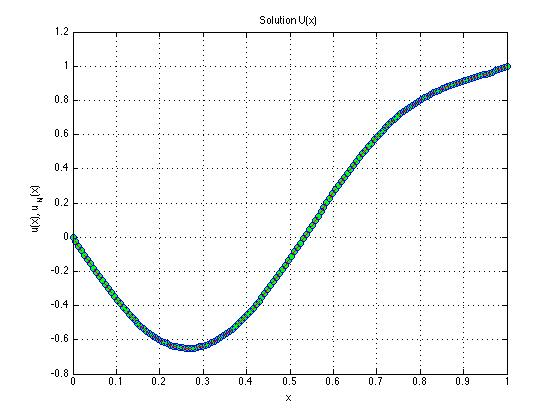
\includegraphics[width=\textwidth]{solutionk2.jpg}
                \caption{solution(k=2)}
                \label{fig:k2}
        \end{subfigure}%
        ~ %add desired spacing between images, e. g. ~, \quad, \qquad, \hfill etc.
          %(or a blank line to force the subfigure onto a new line)
        \begin{subfigure}[b]{0.45\textwidth}
                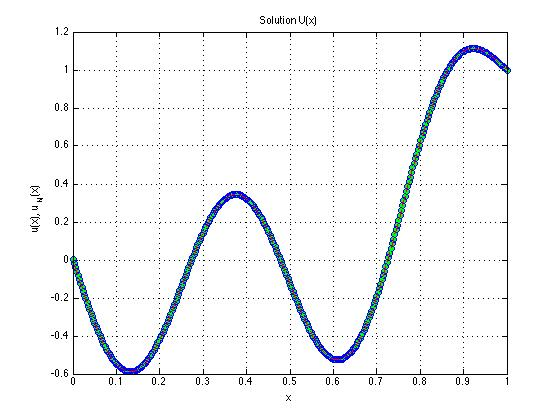
\includegraphics[width=\textwidth]{solutionk4.jpg}
                \caption{solution(k=4)}
                \label{fig:k4}
        \end{subfigure}
        %add desired spacing between images, e. g. ~, \quad, \qquad, \hfill etc.
          %(or a blank line to force the subfigure onto a new line)
        \begin{subfigure}[b]{0.45\textwidth}
                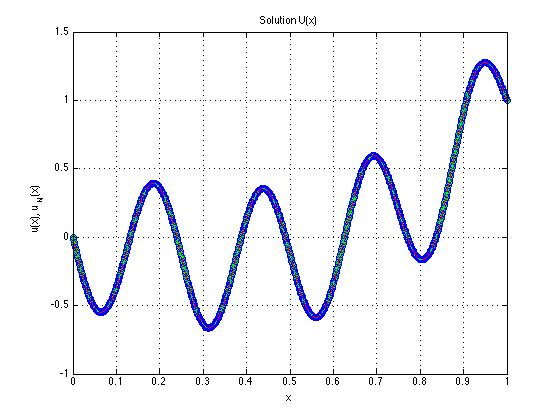
\includegraphics[width=\textwidth]{solutionk8.jpg}
                \caption{solution(k=8)}
                \label{fig:k8}
        \end{subfigure}
        ~ 
         \begin{subfigure}[b]{0.45\textwidth}
                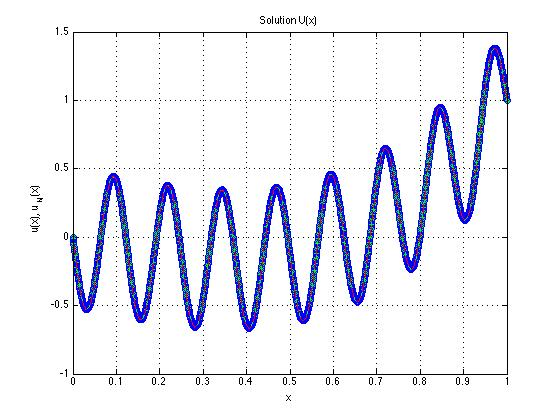
\includegraphics[width=\textwidth]{solutionk16.jpg}
                \caption{solution(k=16)}
                \label{fig:k8}
        \end{subfigure}

        \caption{solution u(x) and $u_N(x)$}\label{fig:solution}
\end{figure}

\begin{figure}
        \centering
        \begin{subfigure}[b]{0.45\textwidth}
                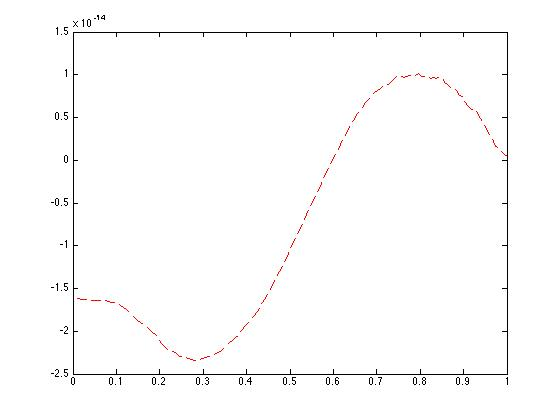
\includegraphics[width=\textwidth]{error2.jpg}
                \caption{error(k=2)}
                \label{fig:k2}
        \end{subfigure}%
        ~ %add desired spacing between images, e. g. ~, \quad, \qquad, \hfill etc.
          %(or a blank line to force the subfigure onto a new line)
        \begin{subfigure}[b]{0.45\textwidth}
                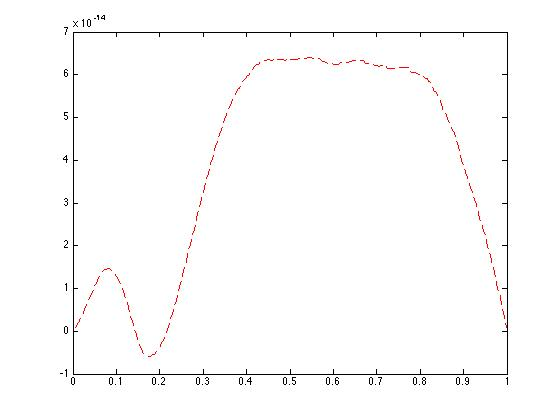
\includegraphics[width=\textwidth]{errork4.jpg}
                \caption{error(k=4)}
                \label{fig:k4}
        \end{subfigure}
        %add desired spacing between images, e. g. ~, \quad, \qquad, \hfill etc.
          %(or a blank line to force the subfigure onto a new line)
        \begin{subfigure}[b]{0.45\textwidth}
                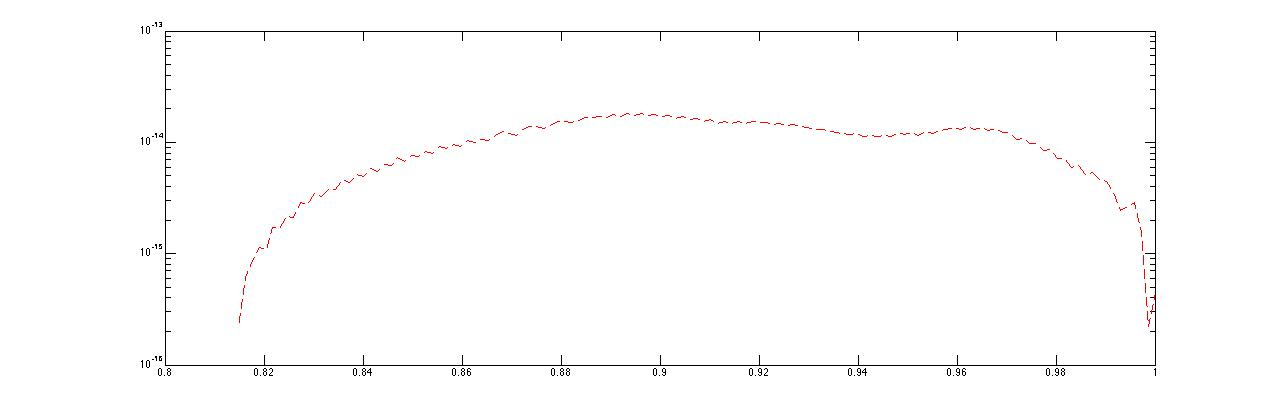
\includegraphics[width=\textwidth]{errork8.jpg}
                \caption{error(k=8)}
                \label{fig:k8}
        \end{subfigure}
        ~ 
         \begin{subfigure}[b]{0.45\textwidth}
                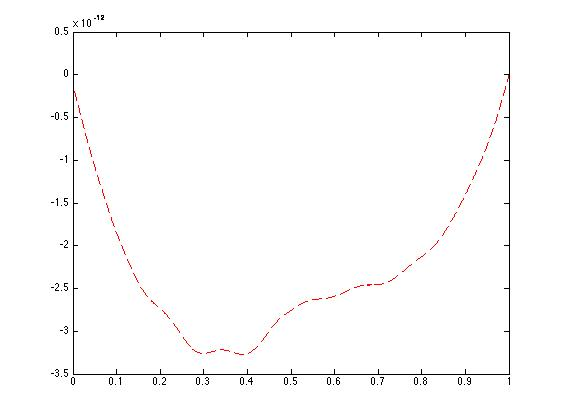
\includegraphics[width=\textwidth]{errork16.jpg}
                \caption{error(k=16)}
                \label{fig:k8}
        \end{subfigure}

        \caption{error between u(x) and $u_N(x)$}\label{fig:error}
\end{figure}




\section{Conclusion}
With the constant k in the right side of the equation getting larger, the frequency of $sin(\pi k x /L)$ increases, so we need more nodes to capture the fluctuation of the solution. The number of elements needed for the same error criteria is almost proportional to k.

Three points gaussian quadriture is used in the project, giving exact integral values for polynomials with order 5 or less. 

Keeping in mind the computation cost is important for engineers. Several technics were used in this project to save the memory and computation cost, such as binary search and sparse matrix. 


\end{document}